\documentclass[12pt]{report}
\usepackage{pdfpages}
\usepackage{lscape}
\usepackage{hyperref}
\hypersetup{
    colorlinks=true,
    linkcolor=black,
    %filecolor=magenta,      
    urlcolor=black,
    breaklinks=true,
   % citecolor=blue,
}
\usepackage[nottoc,notlof,notlot]{tocbibind} 
\usepackage{framed}
\usepackage{rotfloat}
% \usepackage{subfig}
\usepackage[numbers]{natbib}
\usepackage{hyperref}
\usepackage{tabularx}
\usepackage{booktabs}
\usepackage{graphicx}
\usepackage{caption} 
%\captionsetup[table]{skip=10pt}
\usepackage{graphicx}
\usepackage[utf8]{inputenc}
\usepackage{verbatim}
\usepackage[utf8]{inputenc}
\usepackage{amsmath}
\usepackage[english]{babel}
\usepackage{float}
\usepackage{amsthm}
\newtheorem{theorem}{Theorem}
\newtheorem{lemma}{Lemma}
\newtheorem{proposition}{Proposition}
\usepackage{tikz}
\usetikzlibrary{arrows.meta}
\usepackage{tikz}
\usepackage{pgfplots}
\usepackage{pbox}
\usepackage{url}
\usepackage{tkz-graph}
\usetikzlibrary{arrows}
\usepackage{array}
\usepackage{amssymb}
\usepackage{fancyvrb}
\usepackage{listings}
\usepackage{ragged2e}
\usepackage{slashbox}
\makeatletter
\def\BState{\State\hskip-\ALG@thistlm}
\makeatother
\usepackage{sectsty}
\usepackage{comment}
\usepackage{soul}
\usepackage{enumitem}
\usepackage{array}
\usepackage{chngcntr}
\usepackage{cancel}
\usepackage{multirow}
\usepackage{subcaption}
%\usepackage{subfigure}
\usepackage[toc,page]{appendix}
\usepackage{tikz}
\usepackage{setspace}
\usepackage{afterpage}
\usetikzlibrary{shapes,arrows, positioning}
\graphicspath{ {images/} }
%\topmargin -23 mm
\providecommand{\keywords}[1]{\textbf{\textit{Keywords---}} #1}
%\headheight 8pt
%\oddsidemargin 0mm
%\evensidemargin -5mm
\textwidth 161mm
\textheight 210mm
\linespread{1}
%\footskip = 60pt
\usepackage{titlesec}
\chapterfont{\centering}
\newcolumntype{P}[1]{>{\centering\arraybackslash}p{#1}}
\newcolumntype{M}[1]{>{\centering\arraybackslash}m{#1}}
\renewcommand{\baselinestretch}{1.3} 
\titleformat{\chapter}[display]   
{\normalfont\huge\bfseries\centering}{\chaptertitlename\ \thechapter}{10pt}{\Huge\centering}   
\titlespacing*{\chapter}{0pt}{-50pt}{5pt}
\usepackage{pdfpages}
\usepackage[linesnumbered,ruled]{algorithm2e}
\usepackage[  
 top    = 1.5in,
  bottom = 1in,
  left   = 1.5in,
  right  = 1in, 
  %headsep=5mm,%%% Example
  %includeheadfoot%%%%%%%%%%%%%%%%%%%%%%%%%%
  ]{geometry}
%below code used for page bordering
\iffalse
\usepackage{pgf}
\usepackage{pgfpages}0
\pgfpagesdeclarelayout{boxed}
{
  \edef\pgfpageoptionborder{4pt}
}
{
  \pgfpagesphysicalpageoptions
  {%
    logical pages=1,%
  }
  \pgfpageslogicalpageoptions{1}
  {
    border code=\pgfsetlinewidth{1.5pt}\pgfstroke,%
    border shrink=\pgfpageoptionborder,%
    resized width=.95\pgfphysicalwidth,%
    resized height=.95\pgfphysicalheight,%
    center=\pgfpoint{.5\pgfphysicalwidth}{.5\pgfphysicalheight}%
  }%
}
\pgfpagesuselayout{boxed}
\setlength{\parindent}{2cm}
\usetikzlibrary{calc}
\usepackage{eso-pic}
\fi

\begin{document}
\counterwithin{table}{chapter}
\counterwithin{figure}{chapter}
\thispagestyle{empty}
\iffalse
\AddToShipoutPictureBG*{%
\begin{tikzpicture}[overlay,remember picture]
\draw[line width=4pt]
    ($ (current page.north west) + (1cm,-1cm) $)
    rectangle
    ($ (current page.south east) + (-1cm,1cm) $);
\draw[line width=1.5pt]
    ($ (current page.north west) + (1.2cm,-1.2cm) $)
    rectangle
    ($ (current page.south east) + (-1.2cm,1.2cm) $);
\end{tikzpicture}
}
\fi
 \begin{center}
	Major Project Report on\\
	\null
	\textbf{\large \textbf{Learning-Based Log Anomaly Detection, Cryptanalysis, and Design of Image Sharing and Encryption Schemes}}\\
	\null
	
	Submitted in partial fulfillment of the requirements for the degree of\\
	\null
	BACHELOR OF TECHNOLOGY\\
	in\\
	INFORMATION TECHNOLOGY\\
	
	by \\
	\textbf{Sanketh N S (221IT060)}
	\\\textbf{Vrushank T S (221IT083)}
	\\\textbf{{Nithin S (221IT085)}}\\
	\vspace{0.6em}
	\large{\textit{under the guidance of}} \\
	\vspace{0.6em}
	
	\large{\textbf{Dr. Purushothama B R}}\\
	\begin{figure}[h] % b - bottom, t - top, h - here
		\centering{
			
\includegraphics[width=6cm, height=6cm]{symbol.jpg}
		}
	\end{figure}
DEPARTMENT OF INFORMATION TECHNOLOGY\\
NATIONAL INSTITUTE OF TECHNOLOGY KARNATAKA\\
SURATHKAL, MANGALORE - 575025\\

April, 2026\\
\end{center}
\clearpage
\thispagestyle{empty}


\begin{framed}
	\begin{center}
		\textbf{{\Large DECLARATION}}\\ 
\vspace{0.3cm}
        by the B.Tech Student
	\end{center}
	\null
	We hereby \textit{declare} that the Major Project Work Report entitled \textit{\textbf{``Role-Aware Log Anomaly Detection and Learning-Based Security Analysis of Image Sharing and Encryption Schemes''}}, which is being submitted to the \textbf{National Institute of Technology Karnataka, Surathkal}, for the award of the Degree of Bachelor of Technology in Information Technology, is a \textit{bonafide report of the work carried out by us.} The material contained in this Major Project Report has not been submitted to any University or Institution for the award of any degree.
	\\
	\\
	\textit{Name of the Student (Registration Number) with Signature }
	\begin{enumerate}[label={(\arabic*)}]
		\item  Sanketh NS (221IT060)\hspace{0.5em} 
		\item  Vrushank TS (221IT083)
        \item  Nithin S (221IT085)
  
		%\item  Name 3 (ROll No. 3)
	\end{enumerate}
	\null
	Department of Information Technology \\
	Place     : NITK, Surathkal \\
	Date      : 23/04/2026
	\\
	\\
	\\
	\\
	\\
	\\
	\\

\end{framed}
\clearpage

\begin{framed}
	\begin{center}
		\textbf{{\Large CERTIFICATE}}
	\end{center}
	\null
	This is to \textit{certify} that the Major Project Work Report entitled \textit{\textbf{``Role-Aware Log Anomaly Detection and Learning-Based Security Analysis of Image Sharing and Encryption Schemes''}} submitted by \\
	\\
	\textit{Name of the Student (Registration Number)}
	\begin{enumerate}[label={(\arabic*)}]
		\item  Sanketh NS (221IT060)\hspace{0.5em} 
		\item  Vrushank TS (221IT083)
        \item  Nithin S (221IT085)
		%\item  Name 3 (ROll No. 3)
	\end{enumerate}
	as the record of the work carried out by them, is \textit{accepted as the B.Tech. Major Project work report submission} in partial fulfillment of the requirement for the award of the degree of Bachelor of Technology in Information Technology in the Department of Information Technology, NITK Surathkal.
	
	\begin{minipage}{14cm}
		\begin{flushleft}         
			\vspace{2cm}	
			\textbf{Guide Signature with date}\\	
 			Dr. Purushothama B R\\
			Associate Professor\\
			Department of Information Technology  \\
			NITK Surathkal-575025\\ 

\vspace{2cm}

            Chairman - DUGC\\
            Signature With Date and Seal
		\end{flushleft} 
	\end{minipage}
\\
\\
\\
\end{framed}
\thispagestyle{empty}
\clearpage


\pagenumbering{roman}
\newgeometry{top=1in, bottom=1in, left=1.5in, right=1in}
\begin{center}
\textbf{{\Large ABSTRACT}}\\
\begin{center}
\justifying
Log-based anomaly detection is a critical component of ensuring the reliability 
and security of large-scale software systems. Modern systems generate terabytes 
of log data daily, making automated detection of abnormal patterns essential for 
rapid incident response and failure prevention. Existing parsing-free methods such 
as NeuralLog have advanced the state of the art by eliminating dependency on brittle 
log parsers through BERT-based encoding of raw log text. However, these methods 
treat all tokens uniformly through simple averaging of contextual embeddings, 
discarding the structural organization of log messages, and remove numeric tokens 
that carry critical anomaly signals such as HTTP error codes and hardware identifiers. 
This project proposes a novel role-aware representation learning framework that 
addresses these limitations by inducing latent token roles — state, entity, action, 
quantity, and location — automatically from sequence-level anomaly labels, without 
any manual annotation or log parsing. A role induction network assigns a soft 
probability distribution over five role categories to each token, and role-aware 
pooling constructs structured message representations that preserve both semantic 
and structural information. Numeric tokens are explicitly retained to capture 
quantitative anomaly indicators. The framework is evaluated on four public benchmark 
datasets — HDFS, BGL, Thunderbird, and Spirit — achieving F1-scores of 0.98--0.99 
and consistently outperforming NeuralLog and all baseline methods. Ablation studies 
confirm that both role modeling and numeric token preservation contribute 
independently to the observed improvements. The learned token roles align with 
semantic expectations despite being induced solely from anomaly labels, providing 
an interpretable basis for anomaly attribution with negligible computational 
overhead over NeuralLog.

The second objective of this project investigates the vulnerability of XOR-based 
secret image sharing schemes to learning-based reconstruction attacks using 
autoencoders. Classical $n$-out-of-$n$ XOR schemes provide information-theoretic 
security against adversaries holding strict subsets of shares; however, their 
resilience against data-driven models that exploit learned image priors remains 
largely unexplored. This work proposes an encoder--decoder autoencoder framework 
that attempts to reconstruct a secret image from a constrained consecutive subset 
of its XOR-generated shares, without access to cryptographic keys or the remaining 
shares. The model leverages convolutional feature extraction and skip connections 
to recover structural content from the partial observations available to an attacker. 
Reconstruction fidelity is evaluated using PSNR and SSIM across multiple benchmark 
image datasets. Experimental results show that while meaningful reconstruction is 
possible when all shares are available, reconstruction fails under missing-share 
conditions, thereby preserving the theoretical security guarantees of the XOR scheme 
in practical settings.

The third objective of this project focuses on the cryptanalysis of a chaos-based 
medical image encryption scheme under the chosen-plaintext attack (CPA) model. 
The target scheme employs a permutation-diffusion architecture using Arnold's Cat 
Map and a Two-Dimensional Logistic Sine Coupling Map (2D-LSCM). Through structural 
analysis, this work demonstrates that the keystream used in the diffusion stage is 
independent of the plaintext, allowing it to be recovered exactly using a single 
chosen input. Furthermore, the separability of permutation and diffusion stages 
enables complete reconstruction of the permutation mapping using structured probe 
images. By combining these results, the entire encryption process can be inverted 
without knowledge of the secret key. Experimental validation confirms that the 
attack requires only $n+1$ oracle queries for an $n \times n$ image and achieves 
exact plaintext recovery with zero error. These findings reveal fundamental 
weaknesses in chaos-based encryption designs and highlight that statistical measures 
such as entropy and NPCR are insufficient indicators of cryptographic security.

\end{center}
\end{center}

\keywords{Log Anomaly Detection, Role-Aware Representation Learning, Token Role 
Induction, BERT, Parsing-Free Log Analysis, Deep Learning, Transformer, 
Representation Learning, Visual Cryptography, Secret Image Sharing, XOR Secret 
Sharing, Autoencoder, Reconstruction Attack, Adversarial Machine Learning, 
Image Security, Chaos-Based Encryption, Cryptanalysis, Chosen-Plaintext Attack}\\
\clearpage
\restoregeometry
\renewcommand*{\contentsname}{\MakeUppercase{Contents}}
\renewcommand*{\listfigurename}{\MakeUppercase{List of Figures}}
\renewcommand*{\listtablename}{\MakeUppercase{List of Tables}}
\renewcommand{\bibname}{REFERENCES}
\tableofcontents
\clearpage

\begingroup
\addcontentsline{toc}{chapter}{LIST OF FIGURES}
\listoffigures
\clearpage
\endgroup

\begingroup
\addcontentsline{toc}{chapter}{LIST OF TABLES}
\listoftables
\clearpage
\endgroup

\renewcommand{\chaptername}{CHAPTER}
% ===================================================Chapter 1===============================================================
\pagenumbering{arabic} 
% \chapter*{Abbreviations}
\addcontentsline{toc}{chapter}{Abbreviations}

This section provides a list of abbreviations and acronyms used throughout this report. These abbreviations are commonly employed in the fields of cryptography, artificial intelligence, and machine learning, and are intended to enhance clarity and avoid repetition.

\begin{tabbing}
  \hspace{3cm} \= \kill
  AES \> Advanced Encryption Standard \\
  3DES \> Triple Data Encryption Standard \\
  DES \> Data Encryption Standard \\
  CBC \> Cipher Block Chaining \\
  SPN \> Substitution-Permutation Network \\
  IoT \> Internet of Things \\
  VPN \> Virtual Private Network \\
  IV \> Initialization Vector \\
  AI \> Artificial Intelligence \\
  ML \> Machine Learning \\
  DL \> Deep Learning \\
  BiLSTM \> Bidirectional Long Short-Term Memory \\
  BiGRU \> Bidirectional Gated Recurrent Unit \\
  CNN \> Convolutional Neural Network \\
  LSTM \> Long Short-Term Memory \\
  1D CNN \> One-Dimensional Convolutional Neural Network \\
  RNN \> Recurrent Neural Network \\
  Seq2Seq LSTM \> Sequence-to-Sequence Long Short-Term Memory \\
  ANN \> Artificial Neural Network \\
  FCNN \> Fully Connected Neural Network \\
  RF \> Random Forest \\
  NN \> Neural Network \\
  TF-IDF \> Term Frequency–Inverse Document Frequency \\
  IC \> Index of Coincidence \\
  ROUGE \> Recall-Oriented Understudy for Gisting Evaluation \\
  UTF \> Unicode Transformation Format \\
\end{tabbing}

% \clearpage
% ===================================================Chapter 1===============================================================
\chapter{PRELIMINARIES}
\justifying

This chapter introduces the foundational concepts and theoretical background required to understand the methodologies developed in this project. Each concept is explained from first principles before presenting the formal mathematical notation. The three main areas covered are: log-based anomaly detection, secret image sharing, and cryptanalysis of image encryption schemes.

% ─────────────────────────────────────────────────────────────────────────────
\section{Log-Based Anomaly Detection}
% ─────────────────────────────────────────────────────────────────────────────

\subsection{What are System Logs?}

Every time a software application or operating system performs an operation — starting a service, handling a request, encountering an error — it records a brief textual message called a \textbf{log entry}. These messages form a continuously growing record of the system's behavior known as a \textbf{system log}. For example, a web ikserver might produce entries such as:

\begin{quote}
\texttt{[INFO] Connection established from 192.168.1.1} \\
\texttt{[ERROR] Disk write failed: no space left on device} \\
\texttt{[WARN] Authentication attempt failed for user: admin}
\end{quote}

When a system is behaving normally, its logs follow recognizable, repetitive patterns. When something goes wrong — a hardware failure, a security breach, or a software bug — the log patterns deviate from the norm. \textbf{Anomaly detection} is the task of automatically identifying these deviations.

\subsection{Formal Representation}

Formally, each log message $m$ is treated as a sequence of tokens (words or sub-word units):
\[
m = \{ w_1,\, w_2,\, \dots,\, w_T \}
\]
where $T$ is the number of tokens in the message and $w_i$ denotes the $i^{\text{th}}$ token. A \textbf{log sequence} $S$ is a collection of $L$ consecutive log messages observed within a time window:
\[
S = \{ m_1,\, m_2,\, \dots,\, m_L \}
\]

The anomaly detection task is formulated as a \textbf{binary classification} problem. Given a sequence $S$, a detection function $f$ must assign it a label:
\[
f(S) \;\rightarrow\; \{0,\,1\}
\]
where $0$ denotes \emph{normal} behavior and $1$ denotes \emph{anomalous} behavior. The goal is to \emph{learn} $f$ from historical data so that it generalizes to unseen log sequences.

% ─────────────────────────────────────────────────────────────────────────────
\section{Token Embedding and Representation Learning}
% ─────────────────────────────────────────────────────────────────────────────

\subsection{Why Embeddings?}

Machine learning models operate on numbers, not raw text. An \textbf{embedding} is a way of mapping each word or token to a dense numerical vector so that tokens with similar meanings end up close together in vector space. For instance, the tokens \texttt{``error''} and \texttt{``failure''} would ideally have similar vector representations, whereas \texttt{``error''} and \texttt{``timestamp''} would be far apart.

\subsection{Formal Definition}

Each token $w_i$ is mapped to a continuous vector:
\[
e_i = \text{Embed}(w_i) \;\in\; \mathbb{R}^d
\]
where $d$ is the \textbf{embedding dimension} (a hyperparameter, commonly 128 or 256). The full message is then represented as the ordered set of its token vectors:
\[
M = \{ e_1,\, e_2,\, \dots,\, e_T \}
\]

\subsection{Role-Aware Modeling}

Log messages have an internal structure. Within a single message, different tokens play different \emph{roles}: some tokens are keywords (e.g., \texttt{INFO}, \texttt{ERROR}), others are identifiers (e.g., a process ID), and others are numeric values (e.g., a port number). \textbf{Role-aware modeling} explicitly encodes these structural roles alongside the token content, which has been shown to improve the quality of the learned representations.

% ─────────────────────────────────────────────────────────────────────────────
\section{Self-Attention Mechanism}
% ─────────────────────────────────────────────────────────────────────────────

\subsection{Intuition}

Not every token in a log message is equally important for understanding every other token. Consider the message: \texttt{``User admin login failed at port 22.''}  To understand why \texttt{``failed''} is significant, the model needs to pay attention to \texttt{``login''}, not just to adjacent words. The \textbf{self-attention mechanism} allows each token to dynamically focus on — or ``attend to'' — the other tokens that are most relevant to it, regardless of their distance in the sequence.

\subsection{Query, Key, and Value Projections}

For each token embedding $e_i$, three separate linear projections are computed using learned weight matrices $W_Q$, $W_K$, and $W_V$:

\begin{align*}
Q_i &= W_Q\, e_i \quad \text{(Query: what this token is looking for)} \\
K_i &= W_K\, e_i \quad \text{(Key: what this token has to offer)} \\
V_i &= W_V\, e_i \quad \text{(Value: the actual content this token contributes)}
\end{align*}

Intuitively, the query of token $i$ is matched against the keys of all other tokens to decide how much attention to pay to each.

\subsection{Computing Attention}

The raw attention score between token $i$ and token $j$ is the dot product of their query and key vectors, scaled by $\sqrt{d}$ to prevent excessively large values in high dimensions:
\[
\text{Attention}(i,j) = \frac{Q_i\, K_j^{\top}}{\sqrt{d}}
\]

These raw scores are then converted to a probability distribution over all tokens using the \textbf{softmax} function, giving normalized attention weights:
\[
\alpha_{ij} = \frac{\exp\!\bigl(\text{Attention}(i,j)\bigr)}{\displaystyle\sum_{k=1}^{T} \exp\!\bigl(\text{Attention}(i,k)\bigr)}
\]

Note that $\alpha_{ij} \geq 0$ and $\sum_{j} \alpha_{ij} = 1$, so the weights behave like a probability distribution.

\subsection{Contextual Representation}

The final representation of token $i$ is a weighted sum of all value vectors, where tokens with higher attention weights contribute more:
\[
z_i = \sum_{j=1}^{T} \alpha_{ij}\, V_j
\]

The vector $z_i$ is called the \textbf{contextual representation} of token $i$ because it incorporates information from the entire sequence, weighted by relevance. This is fundamentally different from a plain embedding, which carries no information about surrounding context.

% ─────────────────────────────────────────────────────────────────────────────
\section{Secret Image Sharing}
% ─────────────────────────────────────────────────────────────────────────────

\subsection{The Core Idea}

Suppose a highly sensitive image — such as a medical scan or a classified photograph — needs to be stored across multiple servers. Storing the full image on any single server is risky: if that server is compromised, the secret is exposed. \textbf{Secret image sharing (SIS)} solves this by splitting the image into multiple pieces called \textbf{shares}, such that:

\begin{itemize}
    \item Any sufficiently large subset of shares can \emph{perfectly reconstruct} the original image.
    \item Any smaller subset of shares reveals \emph{absolutely nothing} about the original image.
\end{itemize}

This is sometimes called a \textbf{threshold scheme}.

\subsection{The $(k, n)$-Threshold Scheme}

Formally, a $(k, n)$-threshold SIS scheme divides a secret image $S$ into $n$ shares:
\[
\{s_1,\, s_2,\, \ldots,\, s_n\}
\]
with the following guarantees:

\begin{itemize}
    \item \textbf{Reconstruction}: Any $k$ or more shares suffice to reconstruct $S$ exactly.
    \item \textbf{Security}: Any collection of fewer than $k$ shares is statistically independent of $S$ — no information is leaked.
\end{itemize}

For example, in a $(3, 5)$ scheme, the secret is split into 5 shares distributed across 5 servers. Any 3 servers can collaborate to recover the secret, but any 2 servers (even acting together) learn nothing. This provides both \emph{redundancy} (against server failure) and \emph{security} (against server compromise).

\subsection{Security Assumptions and Their Limitations}

The information-theoretic security guarantee above assumes that shares are analyzed \emph{only} through classical combinatorial means. However, modern deep learning models can sometimes extract partial information by detecting subtle statistical patterns across shares — an assumption that this project explicitly tests and challenges.

% ─────────────────────────────────────────────────────────────────────────────
\section{Autoencoders}
% ─────────────────────────────────────────────────────────────────────────────

\subsection{What is an Autoencoder?}

An \textbf{autoencoder} is a neural network trained to reproduce its own input at the output. At first glance this seems trivial — why train a network to copy an input? The key insight is that the network is forced to pass the information through a \textbf{bottleneck}: a hidden layer with far fewer dimensions than the input. To reconstruct the input faithfully despite this bottleneck, the network is forced to learn a \emph{compact, meaningful representation} of the data.

\begin{figure}[h]
\centering
\begin{minipage}{0.8\textwidth}
\centering
\texttt{Input $\xrightarrow{\text{Encoder}}$ Latent Code $\xrightarrow{\text{Decoder}}$ Reconstructed Output}
\end{minipage}
\end{figure}

\subsection{Architecture}

An autoencoder consists of five conceptual stages:

\begin{enumerate}
    \item \textbf{Input Layer}: Receives the raw data (e.g., a flattened image or a sequence of token embeddings).
    \item \textbf{Encoder}: A stack of layers that progressively compresses the input into a lower-dimensional space. Each layer applies a learned linear transformation followed by a nonlinear activation function.
    \item \textbf{Latent Space} (Bottleneck): The compressed representation $\mathbf{z}$ of the input. This is the most information-dense part of the network. A well-trained encoder maps semantically similar inputs to nearby points in latent space.
    \item \textbf{Decoder}: A symmetric stack of layers that expands the latent code back to the original input dimensionality.
    \item \textbf{Output Layer}: Produces the reconstructed input $\hat{x}$.
\end{enumerate}

\subsection{Training Objective}

Autoencoders are trained in an \textbf{unsupervised} fashion — no labels are required. The training objective is to minimize the \textbf{reconstruction error} between the input $x$ and the output $\hat{x}$, typically measured by the Mean Squared Error (MSE):
\[
\mathcal{L}(x, \hat{x}) = \frac{1}{N} \sum_{i=1}^{N} (x_i - \hat{x}_i)^2
\]
where $N$ is the number of elements (e.g., pixels). In the context of this project, autoencoders are used to learn mappings from image shares back to the original secret image, thereby assessing whether the information-theoretic security of SIS schemes holds under deep learning attacks.

% ─────────────────────────────────────────────────────────────────────────────
\section{Image Quality Evaluation Metrics}
% ─────────────────────────────────────────────────────────────────────────────

To evaluate how faithfully a reconstructed image matches the original, two standard metrics are used.

\subsection{Peak Signal-to-Noise Ratio (PSNR)}

\textbf{PSNR} is derived from the MSE between the original and reconstructed images. It is expressed in decibels (dB) and measures the ratio of the maximum possible signal power to the power of the distortion (noise):
\[
\text{PSNR} = 10 \cdot \log_{10}\!\left(\frac{\text{peakval}^2}{\text{MSE}}\right)
\]
where $\text{peakval}$ is the maximum pixel value (255 for 8-bit images). A \textbf{higher PSNR} means the reconstruction is closer to the original. Typical values above 30 dB are considered good quality, while values below 20 dB indicate significant degradation.

\subsection{Structural Similarity Index Measure (SSIM)}

MSE and PSNR treat each pixel independently, which does not always align with human visual perception. \textbf{SSIM} addresses this by comparing images along three perceptual dimensions simultaneously: \emph{luminance} (overall brightness), \emph{contrast} (variation in brightness), and \emph{structure} (spatial patterns of pixel intensities). The result is a score in the range $[0, 1]$:

\begin{itemize}
    \item A value of \textbf{1} indicates the two images are structurally identical.
    \item A value of \textbf{0} indicates no structural similarity whatsoever.
\end{itemize}

SSIM is preferred over PSNR when perceptual quality is important, since two images can have the same MSE but look very different to a human observer.

% ─────────────────────────────────────────────────────────────────────────────
\section{Chaos-Based Image Encryption}
% ─────────────────────────────────────────────────────────────────────────────

\subsection{Motivation}

Medical images and other sensitive visual data must be protected before transmission or storage. Classical block ciphers (such as AES) operate on byte streams and do not exploit the spatial structure of images. \textbf{Chaos-based encryption} offers an alternative: it uses the output of \emph{chaotic dynamical systems} — mathematical systems with deterministic but unpredictable, highly sensitive behavior — as keystreams to scramble image data.

\subsection{Properties of Chaotic Systems Relevant to Cryptography}

A chaotic system is characterized by the following properties that make it attractive for generating cryptographic material:

\begin{itemize}
    \item \textbf{Sensitivity to initial conditions}: Tiny changes in the starting state (even on the order of $10^{-15}$) lead to completely different trajectories. This means the generated sequence is practically unpredictable without knowledge of the exact initial conditions (the key).
    \item \textbf{Ergodicity}: The system visits all regions of its state space over time, ensuring the generated sequence has good statistical coverage.
    \item \textbf{Mixing property}: Nearby initial states quickly spread across the entire state space, contributing to diffusion of information.
\end{itemize}

\subsection{Permutation-Diffusion Architecture}

A typical chaos-based image encryption scheme follows a two-phase structure:

\begin{itemize}
    \item \textbf{Permutation Phase}: The spatial positions of pixels are rearranged using a chaotic map. The content of each pixel remains unchanged, but its location is scrambled. This destroys spatial correlations between adjacent pixels.
    \item \textbf{Diffusion Phase}: The intensity values of pixels are modified using a chaotic keystream, typically via XOR operations. This ensures that a single-pixel change in the plaintext cascades into changes throughout the ciphertext.
\end{itemize}

Together, permutation provides \emph{confusion} and diffusion provides \emph{spreading}, corresponding to Shannon's classical principles of cipher design.

\subsection{Arnold's Cat Map}

The \textbf{Arnold's Cat Map} is a classic area-preserving map used for pixel permutation. For an image of size $n \times n$, it maps each pixel at position $(x, y)$ to a new position $(x', y')$ as follows:
\[
\begin{pmatrix} x' \\ y' \end{pmatrix}
=
\begin{pmatrix} 1 & 1 \\ 1 & 2 \end{pmatrix}
\begin{pmatrix} x \\ y \end{pmatrix}
\bmod\, n
\]

Each application of this map shuffles the pixel positions in a deterministic but seemingly random manner. After a finite number of iterations, the map is periodic — the image returns to its original state — a property exploited both in encryption and in certain cryptanalytic attacks.

\subsection{2D Logistic Sine Coupling Map (2D-LSCM)}

The \textbf{2D Logistic Sine Coupling Map} is a more complex chaotic system designed to overcome the limited chaotic range of simple 1D maps. It generates two interdependent chaotic sequences $\{x_i\}$ and $\{y_i\}$ via:
\[
\begin{cases}
x_{i+1} = \sin\!\bigl(\pi\bigl(4\theta\, x_i(1-x_i) + (1-\theta)\sin(\pi y_i)\bigr)\bigr) \\[6pt]
y_{i+1} = \sin\!\bigl(\pi\bigl(4\theta\, y_i(1-y_i) + (1-\theta)\sin(\pi x_{i+1})\bigr)\bigr)
\end{cases}
\]
where $\theta \in (0, 1)$ is a coupling parameter that controls the balance between the logistic and sine components. The coupling between the two sequences produces a larger and more uniform chaotic range than either component alone. The output sequences serve as keystreams for both permutation and diffusion in the encryption scheme.

% ─────────────────────────────────────────────────────────────────────────────
\section{Cryptanalysis of Image Encryption Schemes}
% ─────────────────────────────────────────────────────────────────────────────

\subsection{What is Cryptanalysis?}

\textbf{Cryptanalysis} is the science of analyzing encryption schemes to find weaknesses that allow an adversary to recover plaintext (or the key) without legitimate access to the secret key. In the context of image encryption, successful cryptanalysis means recovering the original image from its encrypted form.

\subsection{Attack Models}

Different attack models assume different levels of adversary capability. This project focuses primarily on the most powerful standard model:

\subsubsection{Chosen-Plaintext Attack (CPA)}

In a \textbf{Chosen-Plaintext Attack}, the adversary has access to an \emph{encryption oracle}: a black box that, given any image the adversary chooses, returns its encrypted version. Formally:
\[
C = \mathcal{E}(P)
\]
where $P$ is a chosen plaintext image and $C$ is the resulting ciphertext. The adversary selects plaintexts strategically to extract information about the key or the internal structure of the cipher. This is a standard model in modern cryptography — if a cipher cannot withstand a CPA, it is considered insecure.

\subsection{Exploiting Structural Weaknesses}

Many chaos-based image encryption schemes exhibit specific structural weaknesses that make them vulnerable to chosen-plaintext attacks. The two most common weaknesses are described below.

\subsubsection{Keystream Recovery via All-Zero Images}

If the diffusion phase XORs each pixel with a keystream value that is \emph{independent of the plaintext pixel values}, the keystream can be extracted trivially. By encrypting an all-zero image $P = \mathbf{0}$:
\[
C = \mathbf{0} \oplus K = K
\]
the ciphertext directly reveals the keystream $K$. This keystream can then be used to decrypt \emph{any} ciphertext encrypted with the same key.

\subsubsection{Permutation Recovery via Structured Probe Images}

If the permutation and diffusion phases are applied independently (i.e., the permutation does not depend on the pixel values), the permutation mapping can be recovered by encrypting specially crafted probe images. For instance, an image with exactly one non-zero pixel allows the adversary to observe where that pixel lands after permutation. By repeating this process, the full pixel permutation table can be reconstructed.

\subsection{Necessary Conditions for Security Weakness}

An encryption scheme is fully breakable under a CPA if:
\begin{itemize}
    \item The keystream used in diffusion is \textbf{static} (independent of the plaintext), allowing it to be extracted as shown above.
    \item The permutation and diffusion operations are \textbf{independent} of each other and of the plaintext, allowing them to be recovered and reversed separately.
\end{itemize}

When both conditions hold, an adversary can first recover the keystream, then recover the permutation mapping, and thereby reconstruct any plaintext from its ciphertext with full accuracy. This forms the theoretical basis for the cryptanalysis methodology implemented in this project.
%====================================================Chapter 
% ===================================================Chapter 2===============================================================
\chapter{LITERATURE REVIEW}
\justifying

This chapter provides an extensive overview of existing research relevant to the three problem domains discussed in this work. The problem domains include: (i) log-based anomaly detection in distributed systems, (ii) secure image sharing and reconstruction using visual cryptography and learning-based methods, and (iii) cryptanalysis of chaos-based medical image encryption schemes. Although these problem domains address distinct problem contexts, they share common requirements with regard to learning representations from structured or semi-structured data and evaluating system security under advanced adversarial models. As such, this chapter is broadly divided into three sections, each covering one of these problem domains.
%--------------------------------------------------
\section{Anomaly Detection in Logs}

Log anomaly detection has been extensively studied as an important technique in guaranteeing reliability and security in large-scale distributed systems. Initially, researchers applied mining-based techniques to console logs using statistical and clustering-based approaches \cite{xu2009detecting, lou2010mining, makanju2009clustering}. However, such techniques heavily relied on structured log templates. To overcome this problem, researchers developed new techniques such as Drain \cite{he2017drain} and LogCluster \cite{vaarandi2015logcluster} to automatically parse structured log templates. In addition, researchers developed new tools to standardize parsing-based techniques \cite{zhu2019tools}. However, such techniques face challenges in terms of accuracy due to their dependency on parsing-based techniques.

To overcome this problem, learning-based techniques were developed to detect anomalies in logs. DeepLog \cite{du2017deeplog} employed an LSTM neural network to model sequential dependencies in logs to perform anomaly detection by learning to predict the next event in the logs. LogAnomaly \cite{meng2019loganomaly} further improved DeepLog to detect sequential and quantitative anomalies in logs. The problem of performing robust detection in unstable logs has been addressed in \cite{zhang2019robust}. More recently, researchers have proposed new parsing-free techniques such as Log2Vec \cite{meng2020log2vec} and parsing-free anomaly detection frameworks \cite{neurallog2021}. The transformer-based technique has been developed to model logs based on the attention mechanism \cite{vaswani2017attention} and BERT-based contextual embedding techniques \cite{devlin2018bert}. The increasing importance of attention-based and large language models in log analysis is demonstrated by recent works like LAnoBERT \cite{lee2023lanobert}, LogFormer \cite{guo2024logformer}, and several LLM-based parsing studies \cite{wu2023effectiveness, le2023prompt, ma2024llmparser, jiang2024lilac, xu2024divlog, xiao2024logbatcher}. Extensive surveys \cite{landauer2023survey} emphasize the necessity of robust and structurally aware log representation techniques.

\section{Attack on Secure Image Sharing Schemes using Autoencoders}

The concept of secret image sharing was first motivated by the development of classical secret sharing schemes by Shamir \cite{shamir1979share}, which laid a theoretical foundation for secret sharing among multiple parties. Naor and Shamir \cite{naor1995visual} later extended this idea to visual cryptography for images. The main idea is to encode a secret image into a number of shares such that any qualified set of shares will reveal the secret image visually. However, any unqualified subset will reveal nothing. The problem of visual cryptography is that there is a loss in contrast and resolution. 

To address this problem, XOR-based secret image sharing schemes have been proposed. The XOR-based secret image sharing schemes operate on image pixels instead of bits. The XOR-based secret image sharing schemes use Shannon's perfect secrecy concept \cite{shannon1949communication} to guarantee perfect reconstruction of the secret image from all the shares. The XOR-based secret image sharing schemes also guarantee that any subset of shares is statistically independent of the secret image. This ensures that there is zero mutual information between any unqualified subset of shares and the secret image.

However, the security proofs for the XOR-based constructions assume the presence of adversaries without access to structural priors about natural images. Recent deep learning advances contradict this. Convolutional Neural Networks (CNNs) \cite{lecun1998gradient} have shown impressive performance in learning hierarchical spatial representations from image data. Architectural innovations such as batch normalization \cite{ioffe2015batch} improve the stability of the learning process, while encoder-decoder architectures, such as the U-Net \cite{ronneberger2015unet}, enable accurate reconstruction for inverse image problems. Autoencoders, when learned using pixel-wise reconstruction objectives, can extract compact feature representations that can reconstruct structured image information from corrupted images. Moreover, the use of Perceptual Loss functions \cite{johnson2016perceptual} can improve the reconstruction quality for images. The reconstruction quality for such images can be measured using full-reference image similarity measures. The Peak Signal-to-Noise Ratio (PSNR) can measure the pixel-wise fidelity of the reconstruction, while the Structural Similarity Index Measure (SSIM) \cite{wang2004image} can measure the structural similarity between images by comparing the luminance, contrast, and structural information.

In spite of the solid theoretical foundation of secret sharing via XOR and the remarkable advancements in the field of image reconstruction via deep learning methods, only a few works have attempted to explore the possibility of reconstructing the secret image via learning the priors of images and utilizing only certain subsets of the shares generated via XOR operations. Most of the existing works have been dedicated to enhancing the efficiency and robustness of secret image sharing methods and verifying their feasibility rather than testing their robustness against learning-based attacks. This work attempts to bridge this gap and test the robustness of secret image sharing via XOR operations against learning-based attacks and determine whether the secret image can be reconstructed via learning the priors of images and utilizing only certain subsets of the shares generated via XOR operations.

\section{Cryptanalysis of Chaos-Based Image Encryption Schemes}

Chaos-based image encryption has been widely studied due to its ability to achieve strong confusion and diffusion properties using nonlinear dynamical systems. Early work by Fridrich \cite{fridrich1998image} introduced the permutation-diffusion architecture based on chaotic maps, which has since become a standard design paradigm. In this framework, permutation is used to break spatial correlation among pixels, while diffusion ensures that small changes in the plaintext propagate across the ciphertext.

Several schemes have been proposed by combining different chaotic systems. Guan et al. \cite{guan2005chaos} utilized Arnold's Cat Map along with Chen's chaotic system to enhance permutation complexity. Wu et al. \cite{wu2012image} explored logistic maps for both permutation and diffusion processes. Later works incorporated higher-dimensional chaotic systems and hybrid approaches to improve randomness and enlarge the key space \cite{mursi2014image, hua2018lscm, jain2021medical}. These schemes often report strong statistical performance based on metrics such as entropy, correlation coefficients, NPCR, and UACI.

Despite these improvements, a significant body of research has shown that many chaos-based encryption schemes suffer from fundamental security weaknesses. Xie et al. \cite{xie2017cryptanalysis} demonstrated vulnerabilities in permutation-diffusion structures due to insufficient coupling between stages. Cokal and Solak \cite{cokal2009cryptanalysis} showed that certain chaotic image ciphers are vulnerable to known-plaintext and chosen-plaintext attacks. More recent studies \cite{wen2023cryptanalysis, wen2024cryptanalysis, wen2023lin} have emphasized that plaintext-independent keystream generation is a major design flaw, as it allows attackers to recover equivalent keys using simple algebraic analysis.

A recurring issue in many schemes is that the keystream used in the diffusion stage depends only on the secret key and not on the plaintext. This results in a reusable keystream, which is equivalent to a one-time pad used multiple times. Such designs are inherently vulnerable to chosen-plaintext attacks, where specially crafted inputs can be used to extract the keystream and invert the encryption process. Additionally, the separability of permutation and diffusion stages allows attackers to independently recover pixel mappings and value transformations.

The scheme proposed by Jain et al. \cite{jain2021medical}, which combines Arnold's Cat Map with a Two-Dimensional Logistic Sine Coupling Map, represents a recent attempt to improve security for medical image encryption. However, similar to earlier works, it does not incorporate plaintext-dependent key generation or sufficient coupling between stages. This makes it susceptible to structural cryptanalysis.

The present work builds upon these observations and demonstrates a complete chosen-plaintext attack on such a scheme. By recovering the equivalent keystream using a zero plaintext and reconstructing the permutation mapping using structured probe images, the encryption can be fully inverted without knowledge of the secret key. This highlights the gap between statistical security evaluation and actual cryptographic robustness, reinforcing the need for rigorous cryptanalysis in the design of chaos-based image encryption schemes.
%--------------------------------------------------
%====================================================Chapter 3===============================================================
\begin{center}
\justifying
\chapter{Work Done}

This work addresses three complementary security problems spanning system monitoring and cryptographic analysis. First, it proposes a role-aware representation learning framework for log-based anomaly detection that addresses the structural limitations of existing parsing-free methods. The framework operates directly on raw log text without any dependency on log parsers, while explicitly modeling the functional roles of tokens to produce richer and more interpretable log representations. Second, it investigates the vulnerability of XOR-based secret image sharing schemes under learning-based attacks by employing autoencoder architectures to reconstruct images from incomplete share sets. Third, it performs a cryptanalysis of a chaos-based medical image encryption scheme, demonstrating that structural weaknesses such as plaintext-independent keystream generation and separable permutation-diffusion design enable complete decryption under a chosen-plaintext attack.


% ===========================
% PROBLEM 1
% ===========================

\section{Work Done for Problem 1: Role-Aware Log Anomaly Detection}

\subsection{Enhanced Preprocessing}

Unlike NeuralLog~\cite{neurallog2021}, which discards all numeric tokens prior to 
encoding, our preprocessing pipeline retains numeric tokens as first-class vocabulary 
items. Log messages are normalized to lowercase and tokenized using common delimiters 
such as whitespace, colons, and commas. Numeric tokens such as HTTP status codes, 
memory values, retry counts, and block identifiers are preserved, as they frequently 
carry anomaly-relevant signal that uniform removal would destroy.

\begin{figure}[H]
\centering
\vspace{-0.5em}
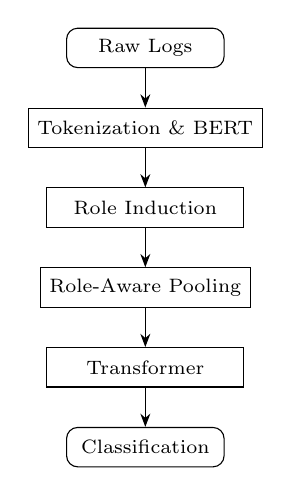
\begin{tikzpicture}[
    node distance=0.5cm,
    startstop/.style={rectangle, rounded corners, minimum width=2cm, minimum height=0.5cm, text centered, draw=black, fill=white!10, font=\scriptsize},
    process/.style={rectangle, minimum width=2.5cm, minimum height=0.5cm, text centered, draw=black, fill=white!5, font=\scriptsize},
    model/.style={rectangle, minimum width=2.5cm, minimum height=0.5cm, text centered, draw=black, fill=white!5, font=\scriptsize},
    arrow/.style={->, >=Stealth}
]
\node (in1) [startstop] {Raw Logs};
\node (pro1) [process, below=of in1] {Tokenization \& BERT};
\node (pro2) [process, below=of pro1] {Role Induction};
\node (pro3) [process, below=of pro2] {Role-Aware Pooling};
\node (mod1) [model, below=of pro3] {Transformer};
\node (out1) [startstop, below=of mod1] {Classification};
\draw [arrow] (in1) -- (pro1);
\draw [arrow] (pro1) -- (pro2);
\draw [arrow] (pro2) -- (pro3);
\draw [arrow] (pro3) -- (mod1);
\draw [arrow] (mod1) -- (out1);
\end{tikzpicture}
\vspace{-0.5em}
\caption{Log Anomaly Detection Pipeline}
\label{fig:architecture}
\end{figure}

\subsection{Token Encoding with BERT}

Each preprocessed log message is tokenized using WordPiece tokenization~\cite{schuster2012japanese}, which decomposes rare or domain-specific terms into frequent subword units, eliminating out-of-vocabulary issues common in technical log vocabularies. Token embeddings are generated using BERT-base (12 layers, 768 hidden dimensions)~\cite{devlin2018bert}, producing a set of contextual representations $\mathbf{H} = [\mathbf{h}_1, \mathbf{h}_2, \ldots, \mathbf{h}_n]$ where each $\mathbf{h}_i \in \mathbb{R}^{768}$ encodes a token in the context of its surrounding message.

\subsection{Latent Token Role Induction}

The central contribution of this work is the latent token role induction mechanism. We postulate that tokens in log messages fulfill distinct functional roles — some denote system states, others identify components, others describe operations, and some convey quantitative or spatial information — and that modeling these roles explicitly produces representations better suited to anomaly detection than uniform averaging.

\subsubsection{Role Categories}

Five latent role categories are defined: \textit{state} (e.g., error, timeout, success), \textit{entity} (e.g., node, disk, process), \textit{action} (e.g., detected, killed, restarted), \textit{quantity} (e.g., error codes, counts, identifiers), and \textit{location} (e.g., file paths, registers, directories). Critically, no manual annotation of these roles is required; they are discovered automatically through end-to-end training on sequence-level anomaly labels.

\subsubsection{Role Induction Network}

For each token $t_i$ with BERT embedding $\mathbf{h}_i \in \mathbb{R}^{768}$, a two-layer feedforward network predicts a soft role distribution: \[ \mathbf{r}_i = \text{softmax}(W_r \cdot \text{ReLU}(W_h \mathbf{h}_i + b_h) + b_r) \] where $W_h \in \mathbb{R}^{256 \times 768}$ and $W_r \in \mathbb{R}^{5 \times 256}$ are learned weight matrices and $\mathbf{r}_i \in \mathbb{R}^5$ is the resulting probability distribution over the five role categories. A role-aware token representation is then formed by modulating the BERT embedding with role information: \[ \mathbf{t}_i = \mathbf{h}_i \odot \mathbf{W}_e \mathbf{r}_i \] where $\mathbf{W}_e \in \mathbb{R}^{768 \times 5}$ is a learned role embedding matrix and $\odot$ denotes element-wise multiplication. Since the role induction network is trained solely from the anomaly detection gradient signal, tokens that contribute similarly to detection automatically receive similar role assignments.

\subsection{Role-Aware Message Representation}

Rather than uniformly averaging all token embeddings as in NeuralLog, we construct a structured message representation by performing separate pooling operations for each role category: \[ \mathbf{m} = [\mathbf{m}_{\text{state}};\, \mathbf{m}_{\text{entity}};\, \mathbf{m}_{\text{action}};\, \mathbf{m}_{\text{quantity}};\, \mathbf{m}_{\text{location}}] \] where each role-specific pool is computed as a soft weighted average: \[ \mathbf{m}_k = \frac{\sum_{i=1}^{n} r_{i,k} \cdot \mathbf{t}_i} {\sum_{i=1}^{n} r_{i,k}} \] and $r_{i,k}$ is the probability that token $i$ belongs to role $k$. The resulting message vector $\mathbf{m} \in \mathbb{R}^{3840}$ concatenates five role-specific sub-vectors of 768 dimensions each, preserving structural distinctions that a single averaged vector would collapse.

\subsection{Sequence Modeling}

Log sequences are constructed using a sliding window of size 20 and step 1, following the protocol of NeuralLog~\cite{neurallog2021}. Sinusoidal positional encodings~\cite{vaswani2017attention} are added to each message representation to inject ordering information: \[ \mathbf{x}_i = \mathbf{m}_i + \mathbf{p}_i \] A single-layer Transformer encoder with 12 attention heads and a feedforward dimension of 2048 is then applied over the sequence to model temporal dependencies among log messages: \[ \mathbf{X}' = \text{TransformerEncoder}(\mathbf{X}) \]

\subsection{Classification and Training}

A max-pooling operation is applied over the sequence output to obtain a fixed-size representation, which is passed through a fully connected layer followed by softmax to produce the anomaly prediction: \[ P(\text{anomaly} \mid \mathbf{s}) = \text{softmax}(W_c \mathbf{s} + b_c) \] The full framework is trained end-to-end using binary cross-entropy loss: \[ \mathcal{L} = -\sum_{j} y_j \log \hat{y}_j + (1 - y_j)\log(1 - \hat{y}_j) \] with the AdamW optimizer at a learning rate of $3 \times 10^{-4}$, a batch size of 64, and a dropout rate of 0.1. Early stopping is applied after 5 epochs without improvement, with a maximum of 20 training epochs. Sequence-level anomaly labels are the only supervision required; token roles emerge entirely through backpropagation.
% ===========================
% PROBLEM 2
% ===========================

\section{Problem 2: Attack on XOR-Based Secure Image Sharing using Autoencoders}

A $(4,4)$ plain random XOR secret sharing scheme was used for all experiments.

For each secret image:
\begin{itemize}
    \item Three shares are generated randomly using independent Bernoulli sampling,
    \item The fourth share is computed as the XOR of the binarized secret image with the first three random shares.
\end{itemize}

Formally, let $S$ denote the binarized secret image and $R_1, R_2, R_3$ denote independent random shares. The fourth share $R_4$ is computed as: \[ R_4 = S \oplus R_1 \oplus R_2 \oplus R_3. \]

This guarantees that: \[ S = R_1 \oplus R_2 \oplus R_3 \oplus R_4. \]

Under classical cryptographic assumptions, any strict subset of fewer than four shares is information-theoretically insufficient to deterministically recover the secret. All shares are generated dynamically during training to prevent memorization and ensure statistical variability across epochs.

\begin{figure}[H]
\centering
\vspace{-0.5em}
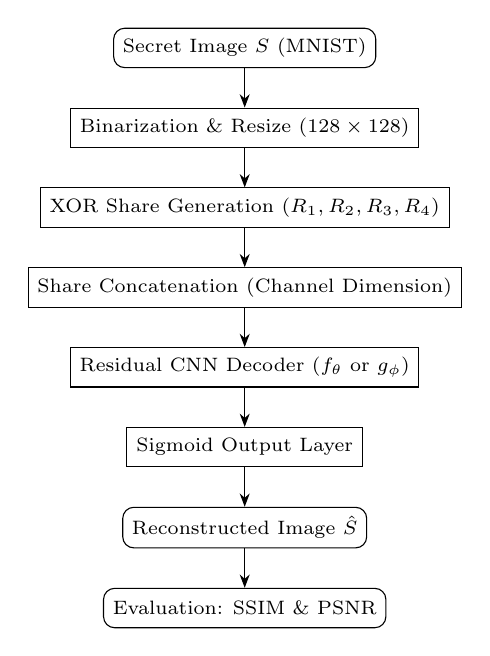
\begin{tikzpicture}[
    node distance=0.5cm,
    startstop/.style={rectangle, rounded corners, minimum width=3cm, minimum height=0.5cm, text centered, draw=black, fill=white!10, font=\scriptsize},
    process/.style={rectangle, minimum width=3cm, minimum height=0.5cm, text centered, draw=black, fill=white!5, font=\scriptsize},
    model/.style={rectangle, minimum width=3cm, minimum height=0.5cm, text centered, draw=black, fill=white!5, font=\scriptsize},
    arrow/.style={->, >=Stealth}
]

% Nodes
\node (in1) [startstop] {Secret Image $S$ (MNIST)};
\node (pro1) [process, below=of in1] {Binarization \& Resize ($128 \times 128$)};
\node (pro2) [process, below=of pro1] {XOR Share Generation ($R_1, R_2, R_3, R_4$)};
\node (pro3) [process, below=of pro2] {Share Concatenation (Channel Dimension)};
\node (mod1) [model, below=of pro3] {Residual CNN Decoder ($f_\theta$ or $g_\phi$)};
\node (pro4) [process, below=of mod1] {Sigmoid Output Layer};
\node (out1) [startstop, below=of pro4] {Reconstructed Image $\hat{S}$};
\node (eval) [startstop, below=of out1] {Evaluation: SSIM \& PSNR};

% Arrows
\draw [arrow] (in1) -- (pro1);
\draw [arrow] (pro1) -- (pro2);
\draw [arrow] (pro2) -- (pro3);
\draw [arrow] (pro3) -- (mod1);
\draw [arrow] (mod1) -- (pro4);
\draw [arrow] (pro4) -- (out1);
\draw [arrow] (out1) -- (eval);

\end{tikzpicture}
\vspace{-0.5em}
\caption{Learning-Based Attack Pipeline on XOR Secret Sharing Scheme}
\label{fig:xor_attack_pipeline}
\end{figure}

\subsection{Dataset Preparation}

The MNIST dataset was used for training and evaluation. All images were:
\begin{itemize}
    \item Normalized to the range $[0,1]$,
    \item Resized to a spatial resolution of $128 \times 128$,
    \item Treated as single-channel grayscale inputs.
\end{itemize}

Share generation was performed on-the-fly during training to prevent fixed share–image pair memorization and to improve generalization of the learning-based decoder.

\subsection{Learning-Based Reconstruction Framework}

To evaluate the vulnerability of XOR-based secret sharing under learning-based
attacks, two distinct decoder configurations were investigated.

\subsubsection{Configuration 1: Decoder Trained on All Four Shares}

In the first configuration, the neural decoder is trained using all four shares as input.

\paragraph{Input Representation}
The four generated shares are concatenated along the channel dimension to form a 4-channel tensor of size $128 \times 128 \times 4$.

\paragraph{Training Objective}
The decoder learns a mapping: \[ f_\theta : \mathbb{R}^{128 \times 128 \times 4} \rightarrow \mathbb{R}^{128 \times 128}, \] where the target output is the original secret image. Binary cross-entropy loss is used for optimization, and the model is trained for 20 epochs using the Adam optimizer.

\paragraph{Evaluation Scenarios}
The trained model is evaluated under multiple share availability conditions:
\begin{itemize}
    \item All four shares available,
    \item One share missing (replaced with a zero/blank share),
    \item Two shares missing (replaced with zero shares),
    \item Three shares missing (only one share available).
\end{itemize}

This configuration models an attacker who has full exposure during training but encounters incomplete share availability during inference.

\subsubsection{Configuration 2: Decoder Trained on Three Consecutive Shares}

In the second configuration, the decoder is trained using only three consecutive shares without wrap-around. The valid combinations considered are:
\begin{itemize}
    \item Shares $\{1,2,3\}$,
    \item Shares $\{2,3,4\}$.
\end{itemize}

\paragraph{Input Representation}
The selected three shares are concatenated to form a 3-channel tensor of size
$128 \times 128 \times 3$.

\paragraph{Training Objective}
The decoder learns the mapping:
\[ g_\phi : \mathbb{R}^{128 \times 128 \times 3} \rightarrow \mathbb{R}^{128 \times 128}. \]

The same residual convolutional architecture, optimizer, and loss function are used as in configuration 1, ensuring architectural consistency across experiments.

\paragraph{Evaluation}
Each consecutive combination is evaluated independently on unseen test images using the same three-share configuration employed during training. This setup models a constrained adversarial scenario in which the attacker never observes all four shares, even during training.

\subsection{Decoder Architecture}

Both configurations employ a convolutional neural network with residual
connections. The architecture consists of:
\begin{itemize}
    \item Initial convolutional layers for low-level feature extraction,
    \item Multiple residual blocks to preserve spatial information and stabilize
    training,
    \item Batch normalization and dropout for regularization,
    \item A sigmoid-activated output layer producing the reconstructed image.
\end{itemize}

The only architectural difference between configuration 1 and configuration 2 lies in the number of input channels (four versus three).

\subsection{Training and Evaluation Protocol}

All models were trained for 20 epochs using dynamically generated share sets
and optimized with the Adam optimizer using binary cross-entropy loss.

Reconstruction quality was evaluated on unseen test images using:
\begin{itemize}
    \item Structural Similarity Index Measure (SSIM),
    \item Peak Signal-to-Noise Ratio (PSNR).
\end{itemize}

Evaluation was performed independently for each share configuration.

\subsection{Outcome}

The experiments demonstrate that neural networks can learn to approximate the
reconstruction function of XOR-based secret sharing without explicitly performing
XOR operations during inference.

While exact reconstruction theoretically requires all four shares, the learning-
based decoder is capable of producing perceptually meaningful approximations even
under partial share availability. This behavior arises from the model exploiting
dataset priors rather than breaking the underlying cryptographic construction.

These findings extend classical cryptographic analysis by highlighting potential
learning-based vulnerabilities when secret sharing schemes are deployed in data-
rich environments.
 The valid combinations considered are:
\begin{itemize}
    \item Shares $\{1,2,3\}$,
    \item Shares $\{2,3,4\}$.
\end{itemize}

\paragraph{Input Representation}
The selected three shares are concatenated to form a 3-channel tensor of size
$128 \times 128 \times 3$.

\paragraph{Training Objective}
The decoder learns the mapping:
\[ g_\phi : \mathbb{R}^{128 \times 128 \times 3} \rightarrow \mathbb{R}^{128 \times 128}. \]

The same residual convolutional architecture, optimizer, and loss function are used as in configuration 1, ensuring architectural consistency across experiments.

\paragraph{Evaluation}
Each consecutive combination is evaluated independently on unseen test images using the same three-share configuration employed during training. This setup models a constrained adversarial scenario in which the attacker never observes all four shares, even during training.

\subsection{Decoder Architecture}

Both configurations employ a convolutional neural network with residual
connections. The architecture consists of:
\begin{itemize}
    \item Initial convolutional layers for low-level feature extraction,
    \item Multiple residual blocks to preserve spatial information and stabilize
    training,
    \item Batch normalization and dropout for regularization,
    \item A sigmoid-activated output layer producing the reconstructed image.
\end{itemize}

The only architectural difference between configuration 1 and configuration 2 lies in the number of input channels (four versus three).

\subsection{Training and Evaluation Protocol}

All models were trained for 20 epochs using dynamically generated share sets
and optimized with the Adam optimizer using binary cross-entropy loss.

Reconstruction quality was evaluated on unseen test images using:
\begin{itemize}
    \item Structural Similarity Index Measure (SSIM),
    \item Peak Signal-to-Noise Ratio (PSNR).
\end{itemize}

Evaluation was performed independently for each share configuration.


% ===========================
% PROBLEM 3
% ===========================

\section{Work Done for Problem 3: Cryptanalysis of Medical Image Encryption Scheme}

This work performs a complete cryptanalysis of a chaos-based medical image encryption scheme proposed by Jain et al.~\cite{jain2021medical}. The scheme employs a permutation-diffusion structure using Arnold's Cat Map and a Two-Dimensional Logistic Sine Coupling Map (2D-LSCM). We demonstrate that the two-round permutation-diffusion structure provides no actual resistance to a chosen-plaintext adversary. Both the equivalent keystream and the full permutation mapping can be extracted with a small oracle query budget, after which any ciphertext may be decrypted without the secret key.

% -----------------------------------------------------------------------
\subsection{Overview of the Target Encryption Scheme}

Two distinct chaotic maps form the algorithmic backbone of the scheme. Arnold's Cat Map handles pixel-position shuffling during the permutation phase, while the Two-Dimensional Logistic Sine Coupling Map (2D-LSCM) drives keystream generation for the diffusion phase.

\subsubsection{Two-Dimensional Logistic-Sine-Coupling Map (2D-LSCM)}

The 2D-LSCM is constructed by coupling the one-dimensional logistic map with the one-dimensional sine map. The logistic map is given by
\begin{equation}
x_{i+1} = r x_i(1-x_i),
\end{equation}
where $r$ denotes the growth-rate parameter and $x_i \in (0,1)$. The sine map takes the form
\begin{equation}
x_{i+1} = \alpha \sin(\pi x_i),
\end{equation}
with control parameter $\alpha \in [0,1]$. Coupling these two one-dimensional systems through a sine nonlinearity produces the 2D-LSCM:
\begin{equation}
\begin{cases}
x_{i+1} = \sin\!\bigl(\pi\bigl(4\theta\, x_i(1-x_i) + (1-\theta)\sin(\pi y_i)\bigr)\bigr),\\[4pt]
y_{i+1} = \sin\!\bigl(\pi\bigl(4\theta\, y_i(1-y_i) + (1-\theta)\sin(\pi x_{i+1})\bigr)\bigr),
\end{cases}
\end{equation}
where $\theta \in [0,1]$ is the coupling control parameter. By operating in a substantially higher-dimensional phase space than either constituent map, the 2D-LSCM achieves greater ergodicity and a wider chaotic parameter range.

\subsubsection{Arnold's Cat Map}

Arnold's Cat Map is a classical area-preserving automorphism of the torus, which, when applied to a square image, performs a deterministic reordering of pixel coordinates. For an image of size $n \times n$, the transformation is
\begin{equation}
\begin{pmatrix} x' \\ y' \end{pmatrix}
=
\begin{pmatrix} 1 & 1 \\ 1 & 2 \end{pmatrix}
\begin{pmatrix} x \\ y \end{pmatrix} \mod n,
\end{equation}
with $(x,y)$ and $(x',y')$ denoting the pre-image and image pixel coordinates, respectively. The mapping is periodic with period $3n+1$, meaning that repeated application returns the image to its original state after exactly $3n+1$ iterations. The number of iterations $P_i$, satisfying $1 < P_i < 3n+1$, constitutes the secret parameter $K_1$ for this component.

% -----------------------------------------------------------------------
\subsection{Encryption Process}

Let $P$ be a plain image of dimensions $M \times N$. Encryption is organized as two consecutive rounds, each comprising a permutation phase followed by a diffusion phase.

\subsubsection{Permutation}

The permutation phase introduces confusion by relocating pixel positions under the joint action of both chaotic maps. Arnold's Cat Map is applied for $P_i$ iterations, and a chaotic matrix $X$ is constructed by iterating the 2D-LSCM; column-wise sorting of $X$ then yields a permutation index matrix that governs the final repositioning of pixel values, producing the permuted image $T$. Critically, the permuted image $T$ depends exclusively on $X$ and $P_i$—no pixel value from $P$ influences the permutation itself.

\subsubsection{Diffusion}

The diffusion phase modifies pixel values so that any single-pixel change in the plaintext propagates throughout the ciphertext. Let $T$ be the permuted image and $X$ the chaotic matrix. For an image sequence of length $O$, the encrypted pixel $E_i$ is
\begin{equation}
E_i =
\begin{cases}
P_1 + P_O + P_{O-1} + X_i \bmod F, & i=1,\\[4pt]
P_2 + E_1 + P_O + X_i \bmod F, & i=2,\\[4pt]
T_i + E_{i-1} + E_{i-2} + X_i \bmod F, & i \geq 3,
\end{cases}
\label{eq:diffusion_enc}
\end{equation}
where $F = 255$ for 8-bit imagery and $X_i = \lfloor x_i \times 2^{32} \rfloor$ is the $i$-th element of the scaled chaotic matrix. The recursive dependence on $E_{i-1}$ and $E_{i-2}$ establishes an inter-pixel dependency chain that ensures downstream propagation of any modification. The entire permutation-diffusion cycle is repeated for a second round to yield the final cipher image $C$.

\begin{figure}[H]
\centering
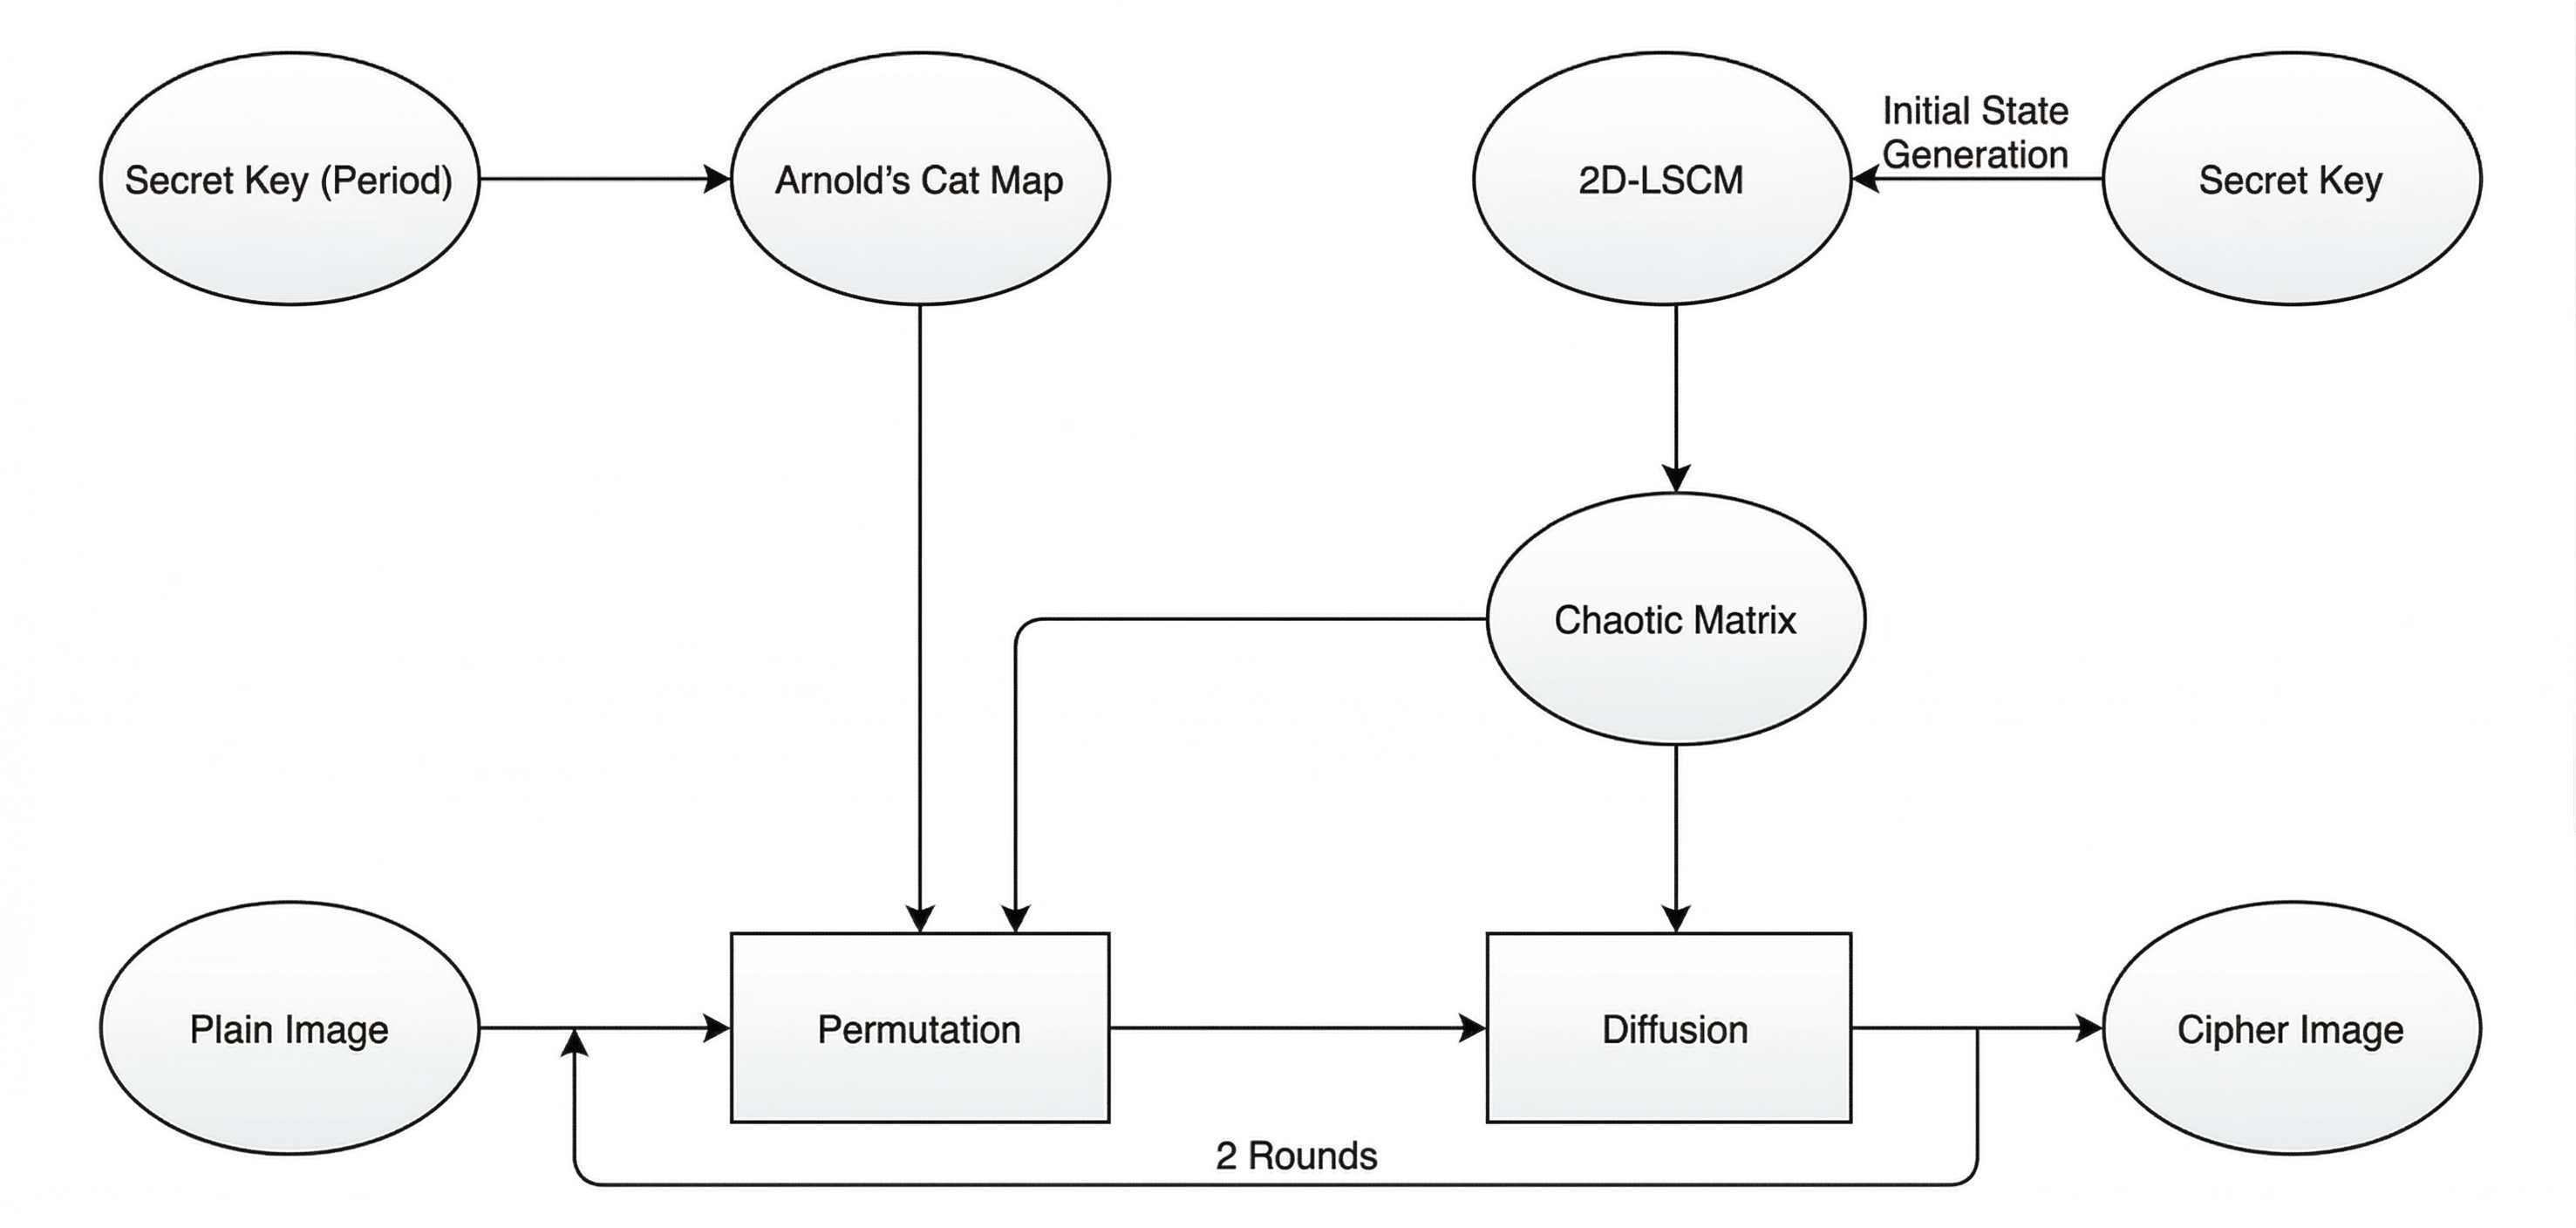
\includegraphics[width=0.9\linewidth]{images/target_methodology.png}
\caption{Encryption process of the target scheme}
\end{figure}

% -----------------------------------------------------------------------
\subsection{Chosen-Plaintext Attack Framework}

The adversary is assumed to have black-box access to an encryption oracle $\mathcal{E}(\cdot)$ that, given any $n \times n$ image $P$, returns the corresponding ciphertext $C = \mathcal{E}(P)$ under an unknown fixed key $(K_1, K_2)$:
\[
C = \mathcal{E}(P).
\]
The adversary has no knowledge of any internal parameters: $x_0$, $y_0$, $\theta$, $P_i$, the chaotic matrix $X$, or the permutation map $\mathcal{M}$.

The exploitable structural weakness is the \emph{plaintext-independence} of all key material. Because the 2D-LSCM sequence $\{x_i\}$ and the derived permutation map $\mathcal{M}$ are functions solely of the secret key—not of the image being encrypted—they remain identical across all images of the same dimensions under the same key. This renders them static equivalent keys, a well-documented vulnerability class in chaos-based cipher design.

The attack proceeds through three phases: (i) keystream extraction by encrypting a zero-valued image, (ii) permutation map reconstruction via structured probe images, and (iii) full decryption of any target ciphertext from the recovered parameters. The data complexity is $n+1$ oracle queries for an $n \times n$ image, and the total computational cost is $\mathcal{O}(n^3)$, dominated by the Arnold map applications in Phase 2.

\begin{figure}[H]
\centering
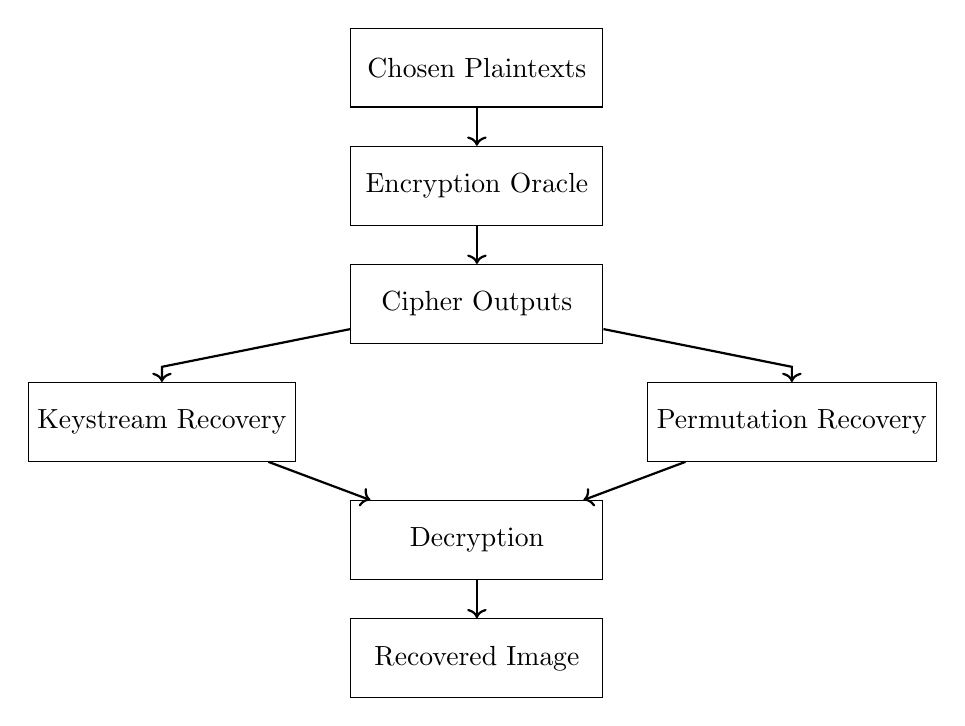
\begin{tikzpicture}[
block/.style={draw, rectangle, minimum width=3.2cm, minimum height=1cm, align=center},
arrow/.style={->, thick}
]
\node[block] (input) at (0,6) {Chosen Plaintexts};
\node[block] (oracle) at (0,4.5) {Encryption Oracle};
\node[block] (cipher) at (0,3) {Cipher Outputs};
\node[block] (ks) at (-4,1.5) {Keystream Recovery};
\node[block] (perm) at (4,1.5) {Permutation Recovery};
\node[block] (decrypt) at (0,0) {Decryption};
\node[block] (out) at (0,-1.5) {Recovered Image};
\draw[arrow] (input) -- (oracle);
\draw[arrow] (oracle) -- (cipher);
\draw[arrow] (cipher) -- (-4,2.2) -- (ks);
\draw[arrow] (cipher) -- (4,2.2) -- (perm);
\draw[arrow] (ks) -- (decrypt);
\draw[arrow] (perm) -- (decrypt);
\draw[arrow] (decrypt) -- (out);
\end{tikzpicture}
\caption{Block diagram of the proposed chosen-plaintext attack showing keystream recovery, permutation recovery, and final decryption without the secret key.}
\label{fig:cpa}
\end{figure}

% -----------------------------------------------------------------------444


\begin{algorithm}[H]
\LinesNumbered
\caption{Chosen-Plaintext Attack on the Target Scheme}
\label{alg:cpa}
\SetAlgoLined
\KwIn{Encryption oracle $\mathcal{E}(\cdot)$; target ciphertext $C$; image size $n$.}
\KwOut{Recovered plaintext $\hat{P}$.}
\BlankLine
\tcp{Phase 1: Keystream Recovery}
$C^{(0)} \leftarrow \mathcal{E}(\mathbf{0}_{n \times n})$ \;
Compute $\hat{X}_i$ for all $i$ using Eq.~\eqref{eq:keystream_recovery}\;
\BlankLine
\tcp{Phase 2: Permutation Map Recovery}
\For{$j = 1$ \KwTo $n$}{
    Construct $P^{(j)}$\;
Set $P^{(j)}_{r,j} \leftarrow r$ for all $r$\;
Set $P^{(j)}_{r,k} \leftarrow 0$ for all $k \neq j$\;

Compute $Q^{(j)} \leftarrow \mathrm{ACM}^{(3n+1-P_i)}\bigl(P^{(j)}\bigr)$\;

$C^{(j)} \leftarrow \mathcal{E}(Q^{(j)})$\;

$\hat{T}^{(j)} \leftarrow \mathcal{D}_{\hat{X}}(C^{(j)})$\;

$\hat{\sigma}_j \leftarrow \hat{T}^{(j)}[:,j]$\;
}
\BlankLine
\tcp{Phase 3: Decryption of Target Ciphertext}
$\hat{T} \leftarrow \mathcal{D}_{\hat{X}}(C)$\;
\For{$j = 1$ \KwTo $n$}{
    $\hat{S}[\hat{\sigma}_j(:),\, j] \leftarrow \hat{T}[:,j]$\;
}
$\hat{P} \leftarrow \mathrm{ACM}^{(3n+1-\tilde{P}_i)}(\hat{S})$\;
\Return $\hat{P}$
\end{algorithm}


\subsection{Phase 1: Keystream Recovery via a Zero Plaintext}

This phase exploits the encryption of an all-zero image to decouple the diffusion layer from the permutation layer and directly expose the keystream.

\subsubsection{Structural Observation}

Let $\mathbf{0}$ denote the $n \times n$ all-zero image and let $C^{(0)} = \mathcal{E}(\mathbf{0})$.

\textbf{Step 1 (Arnold's Cat Map acts as the identity on a zero image).}
Arnold's Cat Map permutes pixel \emph{coordinates} while leaving pixel \emph{values} unchanged. Because every pixel of $\mathbf{0}$ carries the value zero, the map produces the same all-zero image irrespective of the iteration count:
\begin{equation}
\mathrm{ACM}^{P_i}(\mathbf{0}) = \mathbf{0}.
\end{equation}

\textbf{Step 2 (2D-LSCM column permutation acts as the identity on a zero image).}
The column-wise permutation step rearranges rows within column $j$ according to a permutation $\sigma_j$ derived from chaotic matrix $X$. When $P = \mathbf{0}$, every element selected by the permutation equals zero, so:
\begin{equation}
T^{(0)} = \mathbf{0}.
\end{equation}

\textbf{Step 3 (Diffusion collapses to a pure keystream recurrence).}
With $T^{(0)}_i = 0$ for all $i$, the diffusion equation~\eqref{eq:diffusion_enc} simplifies. Substituting and rearranging yields:
\begin{equation}
C^{(0)}_1 = X_1
\end{equation}
\begin{equation}
C^{(0)}_2 = X_1 + X_2 \bmod F
\end{equation}
\begin{equation}
C^{(0)}_i = C^{(0)}_{i-1} + C^{(0)}_{i-2} + X_i \bmod F, \quad i \geq 3.
\end{equation}
Rearranging gives the keystream recovery formula:
\begin{equation}
\boxed{
\hat{X}_i =
\begin{cases}
C^{(0)}_1, & i = 1,\\[4pt]
\bigl(C^{(0)}_2 - C^{(0)}_1\bigr) \bmod F, & i = 2,\\[4pt]
\bigl(C^{(0)}_i - C^{(0)}_{i-1} - C^{(0)}_{i-2}\bigr) \bmod F, & i \geq 3.
\end{cases}
}
\label{eq:keystream_recovery}
\end{equation}

\subsubsection{Correctness of Keystream Recovery}

\begin{proposition}
Every value $\hat{X}_i$ recovered by Eq.~\eqref{eq:keystream_recovery} satisfies $\hat{X}_i = X_i$ for $i = 1, \ldots, N$.
\end{proposition}

\begin{proof}
For $i=1$: directly $\hat{X}_1 = C^{(0)}_1 = X_1$. For $i=2$: $\hat{X}_2 = (C^{(0)}_2 - C^{(0)}_1) \bmod F = X_2$. For $i \geq 3$: by induction, assuming $\hat{X}_k = X_k$ for all $k < i$, we have $\hat{X}_i = (C^{(0)}_i - C^{(0)}_{i-1} - C^{(0)}_{i-2}) \bmod F = X_i$.
\end{proof}

\noindent The complete keystream is thus recovered exactly from a \emph{single} oracle query.

% -----------------------------------------------------------------------
\subsection{Phase 2: Permutation Map Reconstruction}

With the keystream $\{\hat{X}_i\}$ in hand, we reconstruct the full permutation map $\mathcal{M}$ using exactly $n$ additional oracle queries.

\subsubsection{Permutation Structure}

From the encryption process, the permutation stage applies Arnold's Cat Map for $P_i$ iterations and then performs a column-wise sorting step driven by the chaotic matrix $X$. Specifically, for column $j$, if $\sigma_j = \mathrm{argsort}(X[:,j])$ is the permutation induced by sorting that column, the output satisfies
\begin{equation}
T[:,j] = S[\sigma_j, j],
\end{equation}
where $S = \mathrm{ACM}^{P_i}(P)$. The attacker seeks to determine $\mathcal{M}[:,j] = \sigma_j$ for every column.

\subsubsection{Probe Plaintext Design}

For each column index $j \in \{1, \ldots, n\}$, a probe image $P^{(j)}$ is constructed so that column $j$ encodes the row-index sequence $0, 1, \ldots, n-1$ and every other column is identically zero:
\begin{equation}
P^{(j)}_{r,c} =
\begin{cases}
r, & c=j,\\
0, & c \neq j.
\end{cases}
\end{equation}
To neutralize the Arnold preprocessing, the probe submitted to the oracle is the $P_i$-step pre-image of $P^{(j)}$ under the Arnold map, exploiting the map's periodicity:
\begin{equation}
Q^{(j)} = \mathrm{ACM}^{-P_i}\bigl(P^{(j)}\bigr) = \mathrm{ACM}^{(3n+1-P_i)}\bigl(P^{(j)}\bigr).
\end{equation}

\subsubsection{Oracle Output and Permutation Recovery}

When the oracle processes $Q^{(j)}$, the Arnold step undoes the pre-imaging, so that the effective input to the column-sort is precisely $P^{(j)}$. Since column $j$ of $P^{(j)}$ encodes the row indices $r$, the column-sort directly reads out the permutation:
\begin{equation}
T^{(j)}[\ell,j] = \sigma_j(\ell), \qquad \ell = 1, \ldots, n.
\end{equation}
All other columns are zero, so they carry no extraneous information. The oracle then applies diffusion to yield $C^{(j)} = \mathcal{E}(Q^{(j)})$. Inverting the diffusion using the recovered $\hat{X}$:
\begin{equation}
\hat{T}^{(j)}_i =
\begin{cases}
\bigl(C^{(j)}_1 - C^{(j)}_{N} - C^{(j)}_{N-1} - \hat{X}_1\bigr) \bmod F, & i=1,\\[4pt]
\bigl(C^{(j)}_2 - C^{(j)}_1 - C^{(j)}_{N} - \hat{X}_2\bigr) \bmod F, & i=2,\\[4pt]
\bigl(C^{(j)}_i - C^{(j)}_{i-1} - C^{(j)}_{i-2} - \hat{X}_i\bigr) \bmod F, & i \geq 3,
\end{cases}
\label{eq:inv_diff_probe}
\end{equation}
from which the permutation indices for column $j$ are read directly:
\begin{equation}
\hat{\sigma}_j(\ell) = \hat{T}^{(j)}[\ell, j], \qquad \ell = 1, \ldots, n.
\end{equation}
Iterating over all $j = 1, \ldots, n$ completes reconstruction of $\hat{\mathcal{M}}$.

\begin{proposition}
The recovered map satisfies $\hat{\mathcal{M}} = \mathcal{M}$ exactly.
\end{proposition}

\begin{proof}
The probe design guarantees $T^{(j)}[\ell,j] = \sigma_j(\ell)$. Since Proposition~1 guarantees $\hat{X}_i = X_i$ for all $i$, the inverse diffusion in Eq.~\eqref{eq:inv_diff_probe} recovers $\hat{T}^{(j)} = T^{(j)}$ without error, whence $\hat{\sigma}_j = \sigma_j$ for every $j$.
\end{proof}

% -----------------------------------------------------------------------
\subsection{Phase 3: Complete Decryption of Arbitrary Ciphertexts}

Armed with the recovered keystream $\hat{X}$ and permutation map $\hat{\mathcal{M}}$, decryption of any ciphertext $C = \mathcal{E}(P)$ proceeds in three steps without reference to the secret key.

\textbf{Step 1 (Inverse diffusion).}
Compute the permuted image $\hat{T}$ from $C$ via the inverse diffusion operator:
\begin{equation}
\hat{T} = \mathcal{D}_{\hat{X}}(C).
\end{equation}
By Proposition~1, $\hat{T} = T$ exactly.

\textbf{Step 2 (Inverse column permutation).}
For each column $j$, reverse the 2D-LSCM sort using $\hat{\mathcal{M}}$:
\begin{equation}
\hat{S}[\hat{\sigma}_j(\ell),\, j] = \hat{T}[\ell,\, j], \qquad \ell = 1, \ldots, n,
\end{equation}
recovering $\hat{S} = S = \mathrm{ACM}^{P_i}(P)$.

\textbf{Step 3 (Inverse Arnold's Cat Map).}
Apply the Arnold map $(3n+1 - P_i)$ times to $\hat{S}$, exploiting the map's periodicity to compute the inverse via forward iteration:
\begin{equation}
\hat{P} = \mathrm{ACM}^{-P_i}(\hat{S}) = \mathrm{ACM}^{(3n+1-P_i)}(\hat{S}).
\end{equation}
Since $\hat{S} = \mathrm{ACM}^{P_i}(P)$ and Arnold's Cat Map is invertible, $\hat{P} = P$ exactly.

\noindent\textbf{Remark on unknown $P_i$.}
Phase 2 requires knowledge of $P_i$ to construct the probe pre-images $Q^{(j)}$. If $P_i$ is not known, it can be identified by a linear scan: for each candidate $\tilde{P}_i \in \{1, \ldots, 3n\}$, the attacker submits one structured probe and verifies whether column $j$ of the recovered intermediate image matches the expected pattern $\{0,1,\ldots,n-1\}$. The correct value is found in at most $3n - 1$ additional queries, which does not alter the overall polynomial complexity of the attack.

% -----------------------------------------------------------------------
\subsection{Complexity Analysis}

\textbf{Data complexity.}
The entire attack consumes $1 + n$ oracle queries: one zero-image query in Phase 1 and one query per image column in Phase 2. For a $256 \times 256$ image this amounts to 257 queries—negligible from a practical standpoint.

\textbf{Computational complexity.}
Phase 1 inverts the diffusion over all $N = n^2$ pixels in $\mathcal{O}(n^2)$ time. Phase 2 constructs $n$ probe pre-images, each requiring up to $3n$ Arnold map iterations on an $n \times n$ image; since each iteration costs $\mathcal{O}(n^2)$, Phase 2 runs in $\mathcal{O}(n^3)$ in total. Phase 3 requires $\mathcal{O}(n^2)$. The dominant cost is therefore $\mathcal{O}(n^3)$, matching the complexity of the encryption algorithm itself.

\textbf{Memory complexity.}
The attacker need only store the recovered keystream $\hat{X}$ ($n^2$ entries) and the permutation map $\hat{\mathcal{M}}$ ($n^2$ entries), for a total of $\mathcal{O}(n^2)$ space.

%====================================================Chapter 4===============================================================

%===================================================Chapter5=================================================================

%===================================================Chapter6=================================================================

\input{./ref.tex}
\bibliographystyle{IEEEtran}
\bibliography{ref.bib}
\newpage 

% \begin{center}
%     \justifying
%     \centering{\textbf{Publication Details - I}}
% \end{center}

% \vspace{0.5em}
% \begin{itemize}
%     \item The research work has been \textbf{accepted for publication} in the \textbf{6th International Conference on Machine Learning, Image Processing, Network Security and Data Sciences (MIND 2024)}, organized by \textbf{NIT Goa}, India.

%     \item The conference was be held on \textbf{20th and 21st December 2024} at \textbf{NIT Goa}. MIND 2024 is an esteemed international platform that showcases cutting-edge research in \textbf{machine learning, image processing, cybersecurity, and data science}. 

%     \item The paper titled \textit{\textbf{Deciphering Deception: A Dual Approach to Encryption Algorithm Identification and Truth Detection}} has been selected for presentation at the conference and will be published in the official conference proceedings.

%     \item For more information about the conference, please visit the official website: \url{https://mind2024.mind-society.org/} 
% .
% \end{itemize}

% \newpage

% \begin{center}
%     \justifying
%     \centering{\textbf{Publication Details - II}}
% \end{center}

% \vspace{0.5em}
% \begin{itemize}
%     \item The research work carried out as part of this major project has been \textbf{accepted for publication} in the \textbf{3rd International Conference on Networks and Cryptology (NetCrypt 2025)}, organized by the \textbf{School of Computer and Systems Sciences}, Jawaharlal Nehru University (JNU), New Delhi.

%     \item The conference will be held from \textbf{29th to 31st May 2025} at the SC\&SS, JNU, New Delhi. NetCrypt 2025 is a prestigious international platform focusing on the latest advances in \textbf{cryptology, network security, privacy, cyber security, and machine learning}.

%     \item The paper titled \textit{\textbf{AI-Powered Cryptanalysis: Identifying Encryption Algorithms and Recovering Plaintext}} has been selected for presentation at the conference. It will be published in the official conference proceedings. 

%     \item For more details about the conference, please visit the official website: \url{https://www.netcrypt.org.in/}
% \end{itemize}


\end{document}
